\section{Linear-implizite Einschrittverfahren}

Wir haben Verfahren konstruiert, die hohe Ordnung haben, und trotzdem $A$-stabil sind, z.B. das Gauß-Verfahren; es gibt aber noch andere.
Diese Verfahren sind implizit. Zum Berechnen des nächsten Zeitschritts muss ein Gleichungssystem gelöst werden.
\begin{itemize}
	\item Falls $f$ linear ist, so ist dieses Gleichungssystem linear. Das ist okay.
	\item Falls $f$ nichtlinear ist, so ist Gleichungssysteme ebenfalls nichtlinear. Das kann ganz schön teuer werden!
\end{itemize}
Können wir $A$-stabile Verfahren konstruieren, für die bei jedem Schritt nur ein lineares Gleichungssystem gelöst werden muss, selbst wenn $f$ nichtlinear ist?

\subsection{Stabilität von Fixpunkten}

Wir wollen einen alternativen Stabilitätsbegriff für autonome
nichtlineare Differentialgleichungen $x'=f(x)$ untersuchen.

\begin{definition}
	Ein Zustand $x_* \in \Omega_0$ heißt Fixpunkt der Gleichung, wenn $f(x_*)=0$, bzw. wenn $\Phi^tx_* = x_*$ für alle $t$ ist.
\end{definition}
\begin{definition}
	Ein Fixpunkt $x_*$ heißt asymptotisch stabil, wenn ein $\epsilon>0$ existiert, so dass $\lim_{t \to \infty} \Phi^t x_0 = x_*$ für alle $x_0 \in \Omega_0$ mit $\norm{x_* - x_0} < \epsilon$.
\end{definition}

\begin{bsp} ~
	\begin{center}
		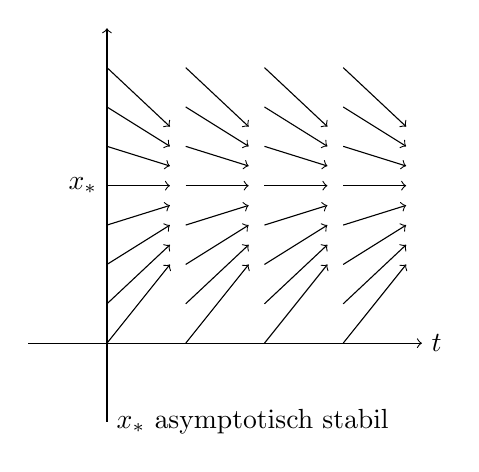
\begin{tikzpicture}
		\draw[->] (0,-1) node[right]{$x_*$ asymptotisch stabil} -- (0,4) ;
		\draw[->] (-1,0) -- (4,0) node[right]{$t$};
		\foreach \i in {0,...,3}
		{
			\foreach \j in {0,...,7}
			{
				\draw[->] (\i,\j / 2) -- (\i + 0.8,\j / 4 + 1) ;
			}
		}
		\draw (0,2) node[left]{$x_*$};
		\end{tikzpicture}
		%
		\hspace{0.1\textwidth}%
		%
		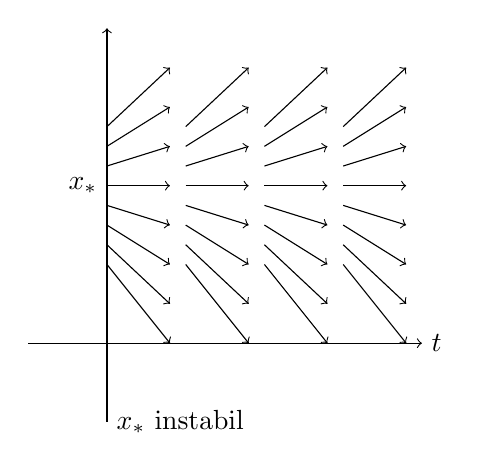
\begin{tikzpicture}
		\draw[->] (0,-1) node[right]{$x_*$ instabil} -- (0,4) ;
		\draw[->] (-1,0) -- (4,0) node[right]{$t$};
		\foreach \i in {0,...,3}
		{
			\foreach \j in {0,...,7}
			{
				\draw[->] (\i,\j / 4 + 1) -- (\i + 0.8,\j / 2) ;
			}
		}
		\draw (0,2) node[left]{$x_*$};
		\end{tikzpicture}
	\end{center}
	Man erkennt an den Bildern, dass die asymptotische Stabilität von $x_*$ mit der Ableitung von $f$ in (der Nähe von) $x_*$ zusammenhängt. 
\end{bsp}


\begin{satz}[{{\cite[3.30]{deuflhard_bornemann:2008}}}]
	Sei $x_* \in \Omega_0$ Fixpunkt von $x' = f(x)$, und $f$ sei stetig differenzierbar. Falls
	\begin{equation*}
	\nu(Df(x_*)) < 0
	\end{equation*}
	so ist $x_*$ asymptotisch stabiler Fixpunkt
\end{satz}

\textbf{Erinnerung:} $\nu$ ist die Spektralabzisse, der größte Realteil aller Eigenwerte.

\textbf{Zwischenfazit:} Um die asymptotische Stabilität von Fixpunkten zu untersuchen, reicht es, sich die Linearisierung um $ x_* $ anzuschauen!

Wir betrachten jetzt zusätzlich die um $ x_* $ linearisierte Differentialgleichung
\begin{equation}\label{Gleichung:Linearisierte-Differentialgleichung}
(x-x_*)' = x' = Df(x_*)(x-x_*).
\end{equation}

\begin{idea}
	Wenn $Df(x_*)$ das Stabilitätsverhalten von $x_*$ qualitativ richtig beschreibt, dann enthält die \emph{lineare} Gleichung~\eqref{Gleichung:Linearisierte-Differentialgleichung}
	vielleicht schon alle \enquote{schwierigen} (im Sinne der Stabilität) Aspekte von $ x'=f(x)$ in der Nähe von $ x_* $?
\end{idea}

Betrachte ein beliebiges Einschrittverfahren. Sei
\begin{itemize}
	\item $\Psi^\tau$ diskreter Fluss für das Ausgangsproblem
	\item $\Psi_*^\tau$ diskreter Fluss für das linearisierte Problem $x'=Df(x_*)(x-x_*)$.
\end{itemize}

\begin{definition}
	Ein Einschrittverfahren heißt \begriff{invariant gegen Linearisierung} um einen Fixpunkt $x_*$, wenn
	\begin{enumerate}
		\item $\Psi^\tau x_*=x_*\ \forall\tau>0$ ($\tau$ zulässig)
		$\qquad \rightarrow$ der Fixpunkt der Differentialgleichung ist auch
		Fixpunkt des numerischen Verfahrens für die nichtlineare Gleichung.
		
		\item $\Psi_*^\tau x = x_* + R(\tau Df(x_*))(x-x_*)$ mit einer rationalen Funktion $R$, die nur vom Verfahren abhängt; d.h. für das linearisierte Problem degeneriert das Verfahren zu einer rationalen Approximation der Exponentialfunktion.
		
		\item $D_x\Psi^\tau x\vert_{x=x_*}=\Psi^\tau_*$ für alle zulässigen $\tau$ $\qquad \rightarrow$ $\Psi^\tau_*$ ist Linearisierung von $\Psi^\tau$.
	\end{enumerate}
\end{definition}

Zum Beispiel sind alle expliziten RK-Verfahren in diesem Sinne invariant. Solch ein Verfahren heißt $A$-stabil, falls $R$ $A$-stabil ist.

Invariante Verfahren retten den Zusammenhang zwischen der asymptotischen Stabilität eines Fixpunkts $x_*$ und der Linearisierung dort ins Diskrete:

\begin{satz}[{{\cite[6.23]{deuflhard_bornemann:2008}}}]
	Sei $\Psi^\tau$, $\Psi^\tau_*$ ein gegen Linearisierung invariantes Einschrittverfahren. Sei $\tau_c\geq 0$ die maximale Schrittweite, so dass $\Psi^\tau_*$ die asymptotische Stabilität erbt. Dann ist $x_*$ asymptotisch stabiler Fixpunkt der Rekursion
	\begin{equation*}
		x_{n+1} = \Psi^\tau x_n\qquad n=0,1,2,\hdots
	\end{equation*}
	für alle $\tau<\tau_c$.
\end{satz}

\begin{bsp}
	Skalare Differentialgleichung $x' = \lambda(1-x^2) \qquad (\lambda > 0)$
	\begin{itemize}
		\item Fixpunkte: $ x_s = 1$ (asymptotisch stabil) und $x_u = -1$ instabil	
		\item Linearisierte Gleichung in $x_s$:
		\begin{equation*}
			x' = f'(x_s)(x-x_s) = -2\lambda x_s(x-x_s) = -2\lambda(x-1)
		\end{equation*}
		\item Explizites Euler-Verfahren dafür stabil, wenn $\tau< 1/\lambda$
		\item Es folgt: $x_s$ ist auch asymptotisch stabiler Fixpunkt des expliziten Euler-Verfahrens für die nichtlineare Gleichung
		\begin{equation*}
			x_{n+1} = x_n + \tau f(x_n) = x_n + \tau\lambda(1-x_n^2).
		\end{equation*}
		Aber wie gesagt nur falls $\tau< 1/\lambda$.
	\end{itemize}
	Und nicht vergessen: $x_s$ ist nur dann Attraktor, wenn man nah genug dran startet. Für dieses Beispiel heißt das:
	\begin{itemize}
		\item Kontinuierlich: $x_0>-1$
		\item Euler: $x_0\in[0, \frac{5}{4}]$.
	\end{itemize}
\end{bsp}

\subsection{Linear-implizite Runge--Kutta-Verfahren}

\begin{idea}
	Behandle nur den linearen Teil von $f$ implizit.
\end{idea}

Für festes $\bar{x} \in \Omega_0$ schreibe die Differentialgleichung als
\begin{equation*}
	x'(t) = Jx(t) + (f(x(t)) - Jx(t)) \qquad J=Df(\bar{x})\in\R^{d\times d}
\end{equation*}
Hier ist $\bar{x}$ beliebig; in der Praxis linearisiert man um den Zustand
zum vorigen Zeitschritt.

Wende das implizite Euler-Verfahren auf den ersten Term an, und das explizite Euler-Verfahren auf den Rest.
\begin{equation*}
\Psi^\tau x = \xi + \tau(f(x)-Jx),\qquad \xi = x+\tau J\xi
\end{equation*}
Das ist das linear-implizite oder \begriff{semi-implizite Euler-Verfahren}.
Wir haben nur ein \textit{lineares} Gleichungssystem pro Schritt, aber sind trotzdem $A$-stabil.

Betrachten wir nun allgemein \begriff{linear-implizite Runge-Kutta-Verfahren}
\begin{equation*}
\Psi^\tau x = x + \tau \sum_{j=1}^s b_j k_j
\end{equation*}
\begin{equation*}
k_i = J\Big(x+\tau\sum_{j=1}^i \beta_{ij} k_j\Big)
+ \bigg[ f\Big(x+\tau\sum_{j=1}^{i-1} \alpha_{ij} k_j\Big)
- J\Big(x+\tau\sum_{j=1}^{i-1} \alpha_{ij} k_j\Big)\bigg]
\end{equation*}
für $i=1,\dots,s$.

\begin{hinw}
	Der obere Summationsindex des impliziten Teils ist $i$, nicht $s$.
\end{hinw}

Dadurch kann der Phasenfluss durch wiederholtes Lösen \textit{linearer} Gleichungssysteme berechnet werden.
\begin{enumerate}
	\item $J = Df(x)$
	\item $\displaystyle (I-\tau\beta_{ii}J)k_i = \tau\sum_{j=1}^{i-1}(\beta_{ij}-\alpha_{ij})Jk_j + f\Big(x + \tau\sum_{j=1}^{i-1} \alpha_{ij} k_j\Big)$ für $i=1,\dots,s$
	\item $\displaystyle \Psi^\tau x = x + \tau\sum_{j=1}^{s} b_j k_j$
\end{enumerate}
Solche Verfahren heißen \begriff{lineare-implizite RK-Verfahren} oder \begriff{Rosenbrock-Verfahren}.


Koeffizienten: $A=(\alpha_{ij})\in\R^{s\times s},\ B=(\beta_{ij})\in\R^{s\times s},\  b=(b_1\hdots,b_s)$

Wählt man die $\beta_{ii}$ alle gleich, so haben die $s$ Gleichungssysteme in (2) alle die gleiche Matrix und es reicht eine LR-Zerlegung, um alle $s$ Gleichungssysteme zu lösen.

Die Frage, ob sich die linearen Gleichungssysteme tatsächlich immer lösen lassen, ist einfacher als für den allgemeinen impliziten Fall:
\begin{lemma}
	Sei $\beta \geq 0$ und $J\in\R^{d\times d}$. Die Matrix $I-\tau\beta J$ ist für alle $0\leq \tau\leq \tau_*$ invertierbar. Dabei hängt $\tau_*$ von der Spektralabzisse $\nu(J)$ ab:
	\begin{equation*}
	\tau_* = \infty\text{ für } \nu(J)\leq 0, \qquad \tau_* =  \frac{1}{\beta\nu(J)} \text{ für }	\nu(J) > 0.
	\end{equation*}
\end{lemma}
\begin{proof}
	Zu zeigen: Unter den gegebenen Voraussetzungen hat $I-\tau\beta J$ nicht den Eigenwert $0$. Nach Satz~\eqref{thm:spektrale_aequivarianz} über rationale Funktionen ist aber
	\begin{equation*}
	\sigma(I-\tau\beta J) = 1-\tau\beta\sigma(J).
	\end{equation*}
	Deshalb zu zeigen: $J$ hat keinen Eigenwert $\lambda$ mit $1-\tau\beta\lambda = 0$.\\
	\begin{enumerate}[label=Fall \arabic*:, leftmargin=*]
		\item $\nu(J) \leq 0$, d.h. insbesondere $\Re(\lambda)\leq 0$:
		\begin{equation*}
		\Re(1-\tau\beta\lambda) = 1-\tau\beta \Re(\lambda) \geq 1 \quad  \Rightarrow \quad 1-\tau\beta\lambda \neq 0
		\end{equation*}
		\item $0<\Re(\lambda)\leq \nu(J)$:
		\begin{equation*}
		\Re(1-\tau\beta\lambda) = 1 - \tau \beta \Re(\lambda) \geq 1 - \tau\beta\nu(J)
		\end{equation*}
		Also $>0$ wenn $\tau < \frac{1}{\beta\nu(J)}$
	\end{enumerate}
\end{proof}

Der Satz sagt also: Die steifen Anteile der Differentialgleichung (d.h. die nichtpositiven Eigenwert von $J$) beeinflussen nicht die Lösbarkeit des Gleichungssystems.

Für autonome \textit{lineare} Probleme ist das Verfahren offensichtlich äquivalent zum impliziten Runge-Kutta-Verfahren $(b, (\beta_{ij}))$.  Es hat also die selbe Stabilitätsfunktion.

Die Konstruktion der Bedingungsgleichungen funktioniert ähnlich wie bei expliziten RK-Verfahren.